\section{Introduction}
Similarity search is widely used in Information Retrieval. For instance, in computer vision such technique is applied to content-based image retrieval (CBIR) so as to search a multimedia collection for images similar to a query.

The larger the document collection is, the smaller the representations should be, in terms of memory consumption. Additionally, a data structure should allow for sublinear-time search in the database of document representations. If the database is so large that the search is computationally infeasible, we can afford making errors as a trade-off for search speed. This concept is called Approximate Nearest Neighbor Search.

If the document representation is a vector in Euclidean space, an exact nearest neighbor search can be performed with methods based on space partitioning, such as k-d tree, R-tree or MVP tree. For an approximate nearest neighbor search a Locality Sensitive Hashing (LSH) technique can be used. Another approach is based on hashing the document representation into binary codes whose properties facilitate the search. In this paper, we will focus on the latter.

In a first part, we will give background information on content-based image retrieval and nearest neighbor search. Furthermore, we will detail the advantages of binary codes for nearest neighbor search. In a second part, we will detail several methods classified in two categories: data independent approaches, which make no prior assumption about the data distribution, and machine learning approaches, which take advantage of the data distribution to optimize the hash function. Finally, in a last part, we will compare the methods in term of hash functions, partitioning of the input space and retrieval performance.

\section{Overview}

\subsection{Content-Based Image Retrieval}
The purpose of content-based image retrieval (CBIR) is to retrieve images by similarity based on a query image. A CBIR system consists of a way of representing an image and a distance, or similarity, measure between two representations. Most approaches to CBIR usually work in two phases: indexing and searching. During the indexing phase, representations of all the images in a collection are extracted and added to a database. The images are not necessarily stored in the database; this reduces its size. Afterward during the searching phase, a query image is presented to the system and its representation is extracted. A nearest neighbor search is then performed with the query representation, using the previously defined distance measure, to search for similar images in the database.

\subsection{Nearest Neighbor Search}
Nearest Neighbor Search is the problem of finding in a database all the items whose distances to a query item are the smallest. Two variants are interesting for CBIR: k-nearest neighbors search and fixed-radius near neighbors. Considering a query point, the former technique aims at finding its k nearest neighbors, whereas the purpose of the latter is to find all points around it within a given radius.

Algorithms such as the k-d tree, R-tree or MVP tree can perform an exact nearest neighbor search. But unfortunately, they are not efficient for high dimensional data. For this reason, Approximate Nearest Neighbors is gaining more interest because it improves searching time with only small actual errors. In any case, we can refine a list of approximate nearest neighbors by pruning the items with the actual distance on the original features.

\subsection{Binary Codes}
Images can be represented with small binary codes (also known as hash codes), which can be compared with a Hamming distance. Because binary codes are small and easy to handle on computers, millions of them can be stored in a database. Furthermore, the whole database can fit in memory, which leads to less IO operations. The Hamming distance can be computed very quickly even on commodity hardware thanks to the POPCOUNT instruction.

To extract a representation of an image in the form of a binary code, we can use a hash function (also known as perceptual hash function). Formally a hash function maps high-dimensional inputs $x\in\mathbb{R}^{p}$, into binary codes, $y\in\mathbb{H}\equiv\{0, 1\}^{q}$, and is defined as: $y=h(x)$. A suitable hash function should map similar (resp. dissimilar) images into similar (resp. dissimilar) binary codes according to a selected distance.

To perform a nearest neighbor search with binary codes two main strategies are to be considered: fast distance approximation and hash table lookup.

By leveraging the fact that the computation of distances between binary codes is fast, we can perform an exhaustive search by computing the distances to all codes in the database. This can be distributed on multiple computers or even on graphics processing units.

The hash table lookup consists in creating a hash table on the binary codes. To perform a nearest neighbor search, we can retrieve the content of the hash buckets in the vicinity of a query code. The complexity, in this case, only depends on the length of binary codes and the search radius. This approach is suited only for small distances because the number of hash buckets within a Hamming ball around a query grows almost exponentially with the search radius. For example, with 32 bits codes and a radius of 8 bits, about 15 million hash buckets are to explore, which is absurd if there are less than 15 million binary codes in the database. \\
A recent approach based on the idea of hash table lookup is Multi Index Hashing \cite{norouzi2012fast}, \cite{norouzi2016}. It consists in building multiple hash tables on binary code sub-strings and yield to sub-linear run-time behavior for uniformly distributed codes.

\section{Approaches}
In this section we will review several approaches. For each of them we will describe the hash function and its associated similarity measure. The hash function determines the partitioning of the input space, which is important to consider. A linear hash function might have more difficulties to preserve similarities of a data set when compared to a non-linear hash function. Non-linear hash functions can more finely discriminate points that are not linearly separable. Moreover non-linear hash functions can discover the internal model of the input space to be able to represent it in a more efficient manner. Hence the binary codes can be shorter without necessarily being less efficient.

There exist different types of hash function: linear transformations, which will be described later, linear transformations followed by a cosine transform, functions based on kernels, functions based on multilayer neural networks, and so on.

One popular hash function is a linear transformation $h_W(x)=thr(Wx)$ where $W\in\mathbb{R}^{q\times{}p}$ and $thr(\cdot)$ is an element-wise Heaviside function. Figure \ref{fig:lsh} shows the partitioning of the space for this particular function. Each row of $W$ denotes the normal of a hyperplane in the input space and determines the value of one bit; 1 is assigned to points on one side of the hyperplane and 0 to points on the other side.

\begin{figure}
	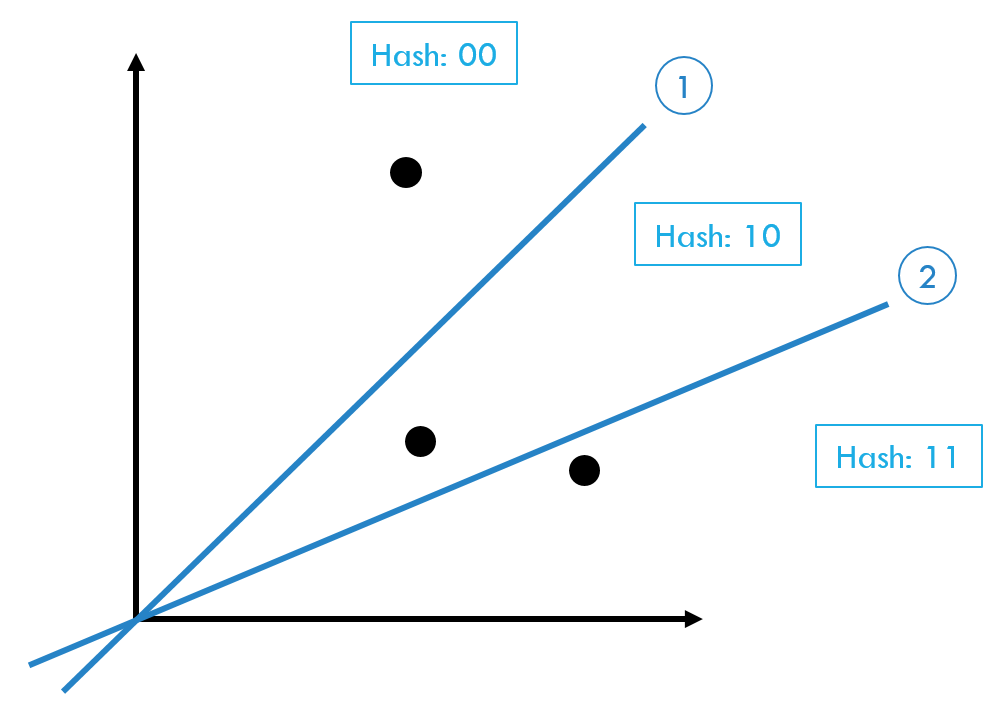
\includegraphics[width=\linewidth]{lsh.png}
	\caption{Partitioning of the space for a hash function based on a linear transformation}
	\label{fig:lsh}
\end{figure}

The most popular similarity measure is based on Hamming distance. Other options are possible: Weighted Hamming distance, Jaccard coefficient, precomputed lookup table, and so on.

Depending on the application and the dimensionality of the inputs and outputs, the complexity of the computation of a hash function can be unacceptable. For example, the computation of q-bit binary codes for a p-dimensional input using a linear transform has a complexity of $O(qp)$. More expressive hash functions can have a higher complexity. Thus, it is important to carefully select the hash function according to the application.

\subsection{Data independent approach}
In this section, we present the data independent approaches, which makes no prior assumption about the data distribution. The most popular approach is based on Locality Sensitive Hashing (LSH) \cite{DBLP:journals/corr/WangSSJ14}. The general idea of LSH is to hash similar input items to the same binary code with higher probability than dissimilar input items. In other words, the goal of LSH is to maximize collisions rather than to avoid them. LSH comes with theoretical guarantees that a specific metric is increasingly well-preserved as the code length increases.

There are different LSH schemes that can preserve different distances: $l_p$ distance, angular distance, Hamming distance, and so on. We will present LSH with random projection which preserves the angular distance.

\subsubsection{Random projection}
~\\
Locality Sensitive Hashing based on random projection \cite{charikar2002similarity} is designed for the angular distance. Thus, it preserves the cosine similarity. The angular distance between two vectors can be computed with

\[similarity=\cos{\theta{}(x_i, x_j)}=\frac{x_i\cdot{}x_j}{\norm{x_i}_2\norm{x_j}_2}\]

\[distance=\frac{\cos^{-1}(similarity)}{\pi}\]

The hash function is defined as $h_W(x)=thr(Wx)$. Each coefficient of W is randomly chosen from a Gaussian distribution. Then the probability of collision is 

\[\mathbb{P}(h_W(x_i)=h_W(x_j))=1-distance=1-\frac{\theta{}(x_i, x_j)}{\pi}\]

It is possible to choose the length of binary codes according to the number of input vectors to hash. According to \cite{DBLP:journals/corr/WangSSJ14}, for $n$ vectors, take $O(\log^2{n})$.

\subsection{Machine learning approach}
In this section, we present the machine learning approach, which takes advantage of the data distribution to optimize the hash function. Two different approaches are detailed, Semantic Hashing is based on an autoencoder, Minimal Loss Hashing and Triplet Loss Ranking, are based on the minimization of a loss function.

In addition to the two main components, hash function and similarity measure, machine learning solutions have an optimization criterion, which defines the objective that the algorithm pursue. A basic optimization criterion is the order-preserving criterion where the results of the ANN search are compared to an external reference. The similarity alignment criterion minimizes the difference between the similarities computed in output and input space. The coding consistent criterion encourages similar (resp. dissimilar) codes when the inputs are similar (resp. dissimilar) and penalizes dissimilar (resp. similar) codes when the inputs are similar (resp. dissimilar). The coding balance criterion aims to uniformly distribute the input vectors among the hash buckets.

In approaches based on machine learning, the parameters of the hash function are optimized using the input data. As usually in machine learning, it is possible to learn the model on a training data set and then use it with other data. A better way to proceed is to use all data to train the model. In this case, over-fitting is not an issue because there is no need to generalize to new data.

While presenting the approaches, we only consider the hash function, the similarity measure and the optimization criterion, without spending too much time on the learning algorithm, assuming that a good solution is found.

\subsubsection{Semantic Hashing}
~\\
Semantic Hashing \cite{salakhutdinov2007semantic},\cite{salakhutdinov2009semantic} is an unsupervised learning approach based on Neural Networks, in fact no similarity information is used. A multilayer autoencoder is used to discover a lower dimensional representation of the input vectors. Its architecture is shown in figure \ref{fig:auto_encoder}. The code layer, which is in the middle of the autoencoder, is forced to use a small number of binary variables (e.g. 32). The model is first pretrained as a stack of RBM's, then it is unrolled to create a multilayer autoencoder, which is fine-tuned by minimizing the root mean squared reconstruction error with backpropagation. To get the final binary code, the activations of the units in the code layer are simply thresholded. With this framework, semantically similar documents are mapped to similar binary codes. Thus, we can use a Hamming distance to compare two binary codes. To perform an approximate nearest neighbor search, rather small codes (e.g. 20 bits) are used and a hash table lookup method is performed with a small radius (e.g. 4 bits). To improve the precision, it is possible to use a two-stage method. At first, a list of candidates is obtained with 28 bits codes, it is then pruned with 256 bits codes.

For the code layer, two technical solutions are available. \\
On the one hand, logistic units are trained with deterministic Gaussian noise. The noise doesn't change during the training, and because there are more examples than parameters in the model, it is forced to generalize rather than to tailor the parameters to the beforehand fixed noise. The presence of noise forces the input of the activation function to be large and negative for some training cases and large and positive for others. Consequently, the noise has only a small impact on the output of the layer. \\
On the other hand, an easier approach discovered later \cite{krizhevsky2011using}. Instead of logistic units, binary stochastic units are used in the code layer and no noise is added. A binary stochastic unit outputs either 1 or 0 otherwise depending on a probability given by a logistic function.

\[z_i=b_i+\sum\nolimits_{j}s_{i}w_{ij}\]
\begin{align*}
\mathbb{P}(s_i=1)=\frac{1}{1+\rm{e}^{-z_i}} && \mathbb{P}(s_i=0)=1-\mathbb{P}(s_i=1)
\end{align*}

To train a binary stochastic unit we pretend during the backpropagation, that the output value comes from a normal logistic unit and it gives a smooth gradient for the backpropagation.

\begin{figure}
	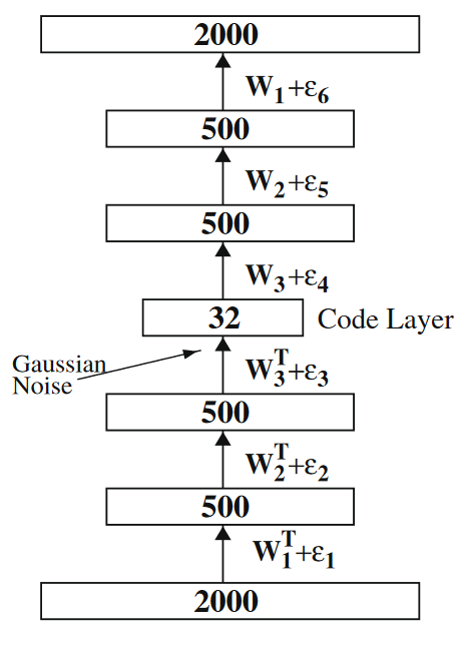
\includegraphics[height=5cm]{auto_encoder.png}
	\caption{Autoencoder in Semantic Hashing}
	\label{fig:auto_encoder}
\end{figure}

\subsubsection{Minimal Loss Hashing}
~\\
Minimal Loss Hashing (MLH) \cite{norouzi2011minimal},\cite{norouzi2016} is a supervised approach based on a hinge-like loss function. A linear hash function is used $h_W(x)=thr(Wx)$, it is also possible to use it with other hash functions as long as they are differentiable with respect to their parameters, so that we can compute the Jacobian. The Hamming distance is used to compare the output binary codes.

The learning is based on a training data set of labeled pairs $(x_i, x'_i, s_i)$ where $x_i$ and $x'_i$ are $p$-dimensional centered training points and $s_i$ is a similarity label, whose value is 1 if $x_i$ and $x'_i$ are similar and 0 if dissimilar. To preserve a specific metric one can compute the similarity label by thresholding the pairwise distance. Alternatively, to preserve the semantic similarity, one can assign a similarity label based on the class label.

For each sample in the training data set, a loss function $l_{pair}: [0, 1]^{q}\times[0, 1]^{q}\times{0, 1}\rightarrow\mathbb{R}^{+}$ assesses the quality of the mapping by assigning a cost to a pair of binary codes and a similarity label. By minimizing the loss over all training examples, we can learn the parameters of the hash function.

\[L(w)=\sum\limits_{i=1}^n l_{pair}(h_W(x_i), h_W(x'_i), s_i)\]

To optimize the parameters of the hash function, the key point of MLH is to use a coding consistent criterion based on a hinge-like loss function. A hyper-parameter $\rho$ is a threshold of distance in Hamming space, that defines the boundary between similar and dissimilar codes. If the distance between two codes is less than (resp. more than) $\rho$ we can consider them as similar (resp. dissimilar). In addition, the $\lambda$ parameter adjusts the penalty incurred for dissimilar pairs when they are too close in comparison to the penalty incurred for similar pairs when they are too far from each other. Although it is a slow process, a good value for these hyper parameters can be found with a validation set. Let $\norm{h - h'}_{H}$ be the Hamming distance between binary codes $h$ and $h'$. The pairwise loss based on the hinge function is defined as:

\[
	l_{hinge}(h, h', s)=
	\begin{cases}
	\max(\norm{h - h'}_{H} - \rho + 1, 0) & \text{for } s=1 \\
	\lambda\max(\rho - \norm{h - h'}_{H} + 1, 0) & \text{for } s=0
	\end{cases}
\]

Minimal Loss Hashing builds a convex-concave upper bound on it. Then a stochastic gradient-based approach is used to minimize the loss function. The learning algorithm is online, scales well to large data sets and large code lengths.

\subsubsection{Triplet Ranking Loss}
~\\
Triplet Ranking Loss (TRL) \cite{norouzi2012hamming},\cite{norouzi2016} is a supervised approach that generalizes Minimal Loss Hashing. While certainly good at learning a metric structure (e.g. Euclidean, Cosine) of the input data, the goal of this approach is rather to preserve the semantic similarity. When no pairwise similarity is available, one could rely on a generic distance (e.g. Euclidean) but this often produce unsatisfactory results. TRL, on the other hand, is based on the relative similarity between a triplet of points. Thus, no pairwise similarity label is required.

A linear hash function is used $h_W(x)=thr(Wx)$, as with MLH it is possible to use other hash functions as long as they are differentiable with respect to their parameters. The Hamming distance is used to compare the output binary codes.

The learning is based on a training data set of triplets of $p$-dimensional centered training points $(x, x^{+}, x^{-})$ such that the pair $(x, x^{+})$ is more similar than the pair $(x, x^{-})$. To build a training data set that preserves semantic similarity one can pick two points from the same class and one point from another class.

As with MLH, for each sample in the training data set, a loss function $l_{rank}: [0, 1]^{q}\times[0, 1]^{q}\times[0, 1]^{q}$ assesses the quality of the mapping by assigning a cost to a triplet of binary codes. The loss function should penalize the examples where $h_W(x_i)$ is closer to $h_W(x^{-}_i)$ than to $h_W(x^{+}_i)$ in Hamming distance. By minimizing the loss over all training examples, we can learn the parameters of the hash function.

\[L(w)=\sum\limits_{i=1}^n l_{rank}(h_W(x_i), h_W(x^{+}_i), h_W(x^{-}_i))\]

To optimize the parameters of the hash function, TRL uses a hinge-like loss function. On the contrary of MLH, there is no hyper parameter, which makes the learning easier because there is no need to find them a good value with a validation set. The loss is zero when $h_W(x_i)$ is closer to $h_W(x^{+}_i)$ than to $h_W(x^{-}_i)$ in Hamming distance. Let $\norm{h - h'}_{H}$ be the Hamming distance between binary codes $h$ and $h'$. In this case, the loss is zero when $\norm{h - h^{+}}_{H}$ is at least one bit smaller than $\norm{h - h^{-}}_{H}$. The triplet loss based on the hinge function is defined as:

\[
	l_{rank}(h, h^{+}, h^{-})=\max(\norm{h - h^{+}}_{H} - \norm{h - h^{-}}_{H} + 1, 0)
\]

The same optimization technique as MLH is used. A convex-concave upper bound is built on the loss function. Then a stochastic gradient-based approach is used to minimize the loss function. TRL is more flexible than the pairwise hinge loss and is shown to produce superior hash functions. A simple kNN classifier on the learned binary codes is competitive with state-of-the-art classifiers on CIFAR and MNIST.

\section{Comparison}
In this section, we will compare the methods in term of hash functions, partitioning of the input space and retrieval performance. We don't take in account the optimization technique of the machine learning approaches, assuming that a good solution is found. 

Fundamentally, data independent approaches should be less efficient than machine learning approaches because they don't take in account the data distribution. This means that on the same instance, depending on the data distribution, the machine learning solutions should generally yield better results. The binary codes generated by data independent approaches should be longer than their equivalent from machine learning approaches for the same retrieval accuracy. The data independent solutions are nevertheless more general and come with theoretical guarantees that a specific metric is increasingly well preserved as the code length increases. Moreover, one has to be very careful when training a machine learning approach because there is many pitfalls: trying to generalize from a bad sampled training data set, making an error during the preprocessing, choosing wrong values for the hyper parameters, choosing, a priori, a hash function that is not appropriate, training only one model and not benchmarking it against other approaches, and so on.

\begin{figure*}
	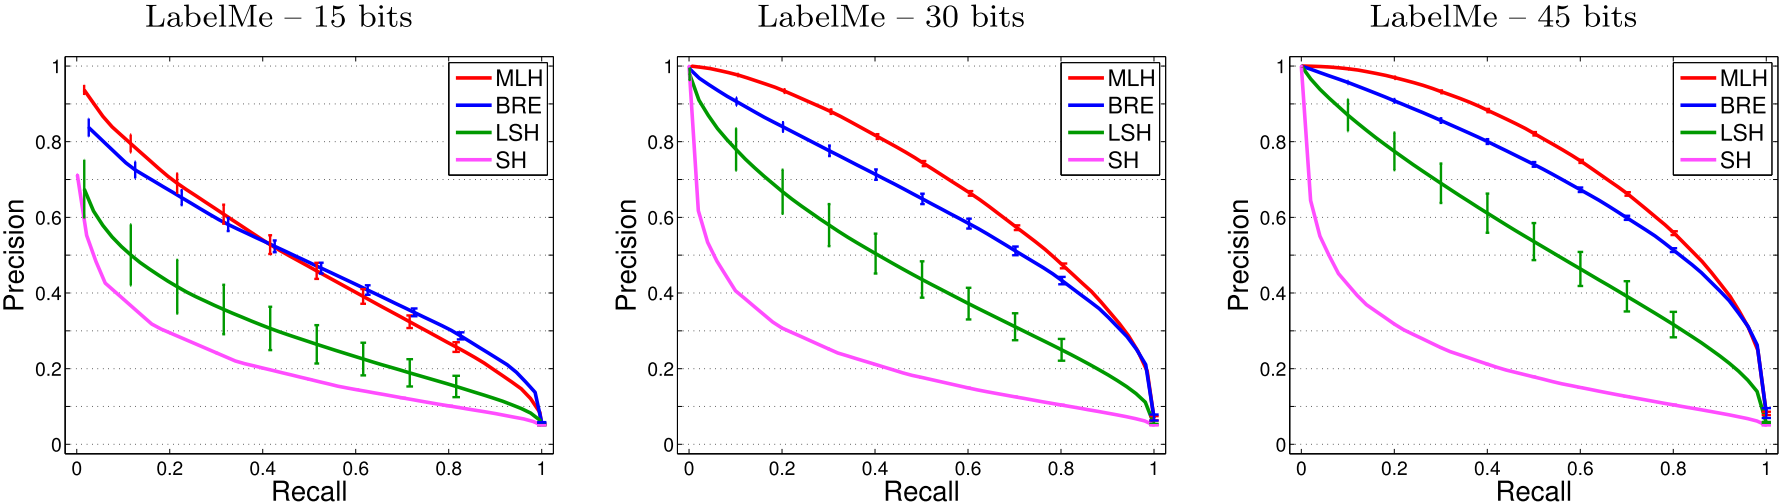
\includegraphics[width=\textwidth]{mlh_labelme.png}
	\caption{Precision-recall curves on LabelMe for different methods for different code lengths. \cite{norouzi2011minimal}}
	\label{fig:mlh_labelme}
	
	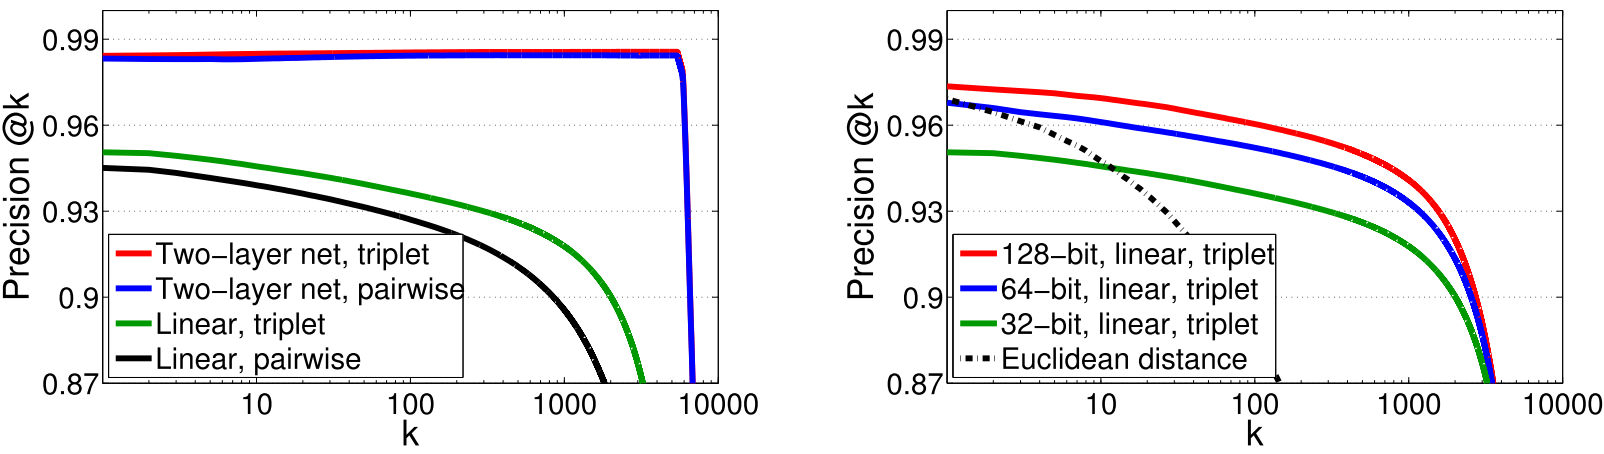
\includegraphics[width=\textwidth]{trl_vs_mlh.png}
	\caption{MNIST precision@k: (left) four methods with 32-bit codes; (right) three code lengths with triplet loss. \cite{norouzi2012hamming}}
	\label{fig:trl_vs_mlh}
\end{figure*}

Based on experiments conducted by the authors of the approaches we can have an idea on their relative performances.

A first experiment, conducted by the authors of Minimal Loss Hashing (MLH) \cite{norouzi2011minimal}, compares it with LSH and other methods. Six data sets are used: \textit{Photo-tourism}, a collection of images represented as 128D SIFT features, \textit{LabelMe} and \textit{Peekaboom}, collections of images represented as 512D Gist descriptors. \textit{MNIST}, a collection of 784D grayscale images of handwritten digits, \textit{Nursery} with 8D features, a synthetic data set comprising uniformly sampled points from a 10D hypercube. All methods used identical training and test sets. The similarity labels are based on a thresholded Euclidean distance so that each point has, on average, 50 neighbors. On each data set, input vectors are mean-centered. On all but the 10D Uniform data set, each datum is normalized. Some methods improve with dimensionality reduction so a PCA is applied to retain 40 dimensions (except for 10D Uniform and 8D Nursery). Average and standard deviation of precision/recall are computed on 10 executions of all methods, except for Spectral Hashing (SH). In this review we only present the precision-recall curves on LabelMe for different code lengths, in figure \ref{fig:mlh_labelme}. Other experiments are conducted in the original paper: precision using a Hamming radius of 3 bits for different methods as a function of code lengths, precision-recall curves for different methods for different code lengths. In almost all cases, the performance of MLH is clearly superior to all others (including LSH).

\begin{figure*}
	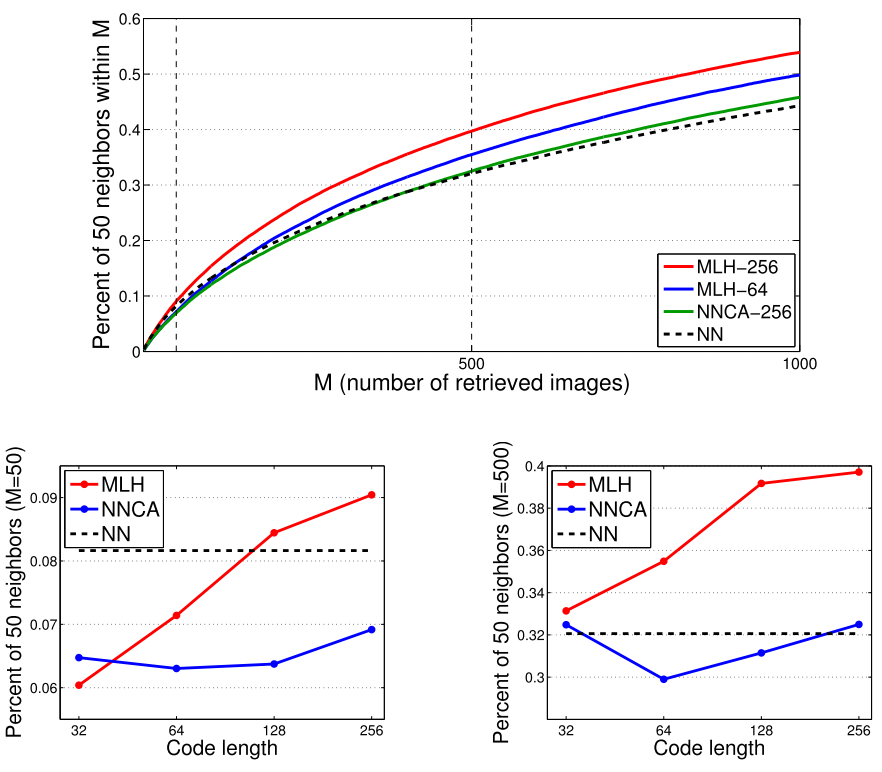
\includegraphics[width=\textwidth]{semantic_search_mlh_nnca.png}
	\caption{(top) Percentage of 50 ground-truth neighbors as a function of number of images retrieved ($0 \leq M \leq 1000$) for MLH with 64, 256 bits, and for NNCA with 256 bits. (bottom) Percentage of 50 neighbors retrieved as a function of code length for $M=50$ and $M=500$. \cite{norouzi2011minimal}}
	\label{fig:semantic_search_mlh_nnca}	
\end{figure*}

A second experiment, conducted by the authors of Triplet Loss Ranking (TRL) \cite{norouzi2012hamming}, compares it with MLH. Two data sets are used, MNIST and CIFAR-10. Similarity labels are derived from class labels: items from the same class are similar. In this review we only present the precision@k (fraction of same-class items from a kNN retrieval) on the MNIST data set for different hash functions, different optimization criteria and for different values of k. The results are plotted in figure \ref{fig:trl_vs_mlh}. The hash function is either a linear transformation or a two-layer neural network. The optimization method is either MLH or TRL. K varies from 1 to 10,000. A Euclidean nearest neighbor search is also included as baseline because it provides an upper bound on the performance of methods that preserve Euclidean distances (e.g. LSH). The conclusion is that TRL yields slightly better performances than MLH.

A third experiment, conducted by the authors of Minimal Loss Hashing (MLH) \cite{norouzi2011minimal}, compares it with NNCA, which is based on Semantic Hashing. The experiment makes use of the 22K LabelMe data set with a semantic pairwise affinity matrix provided by humans. As a consequence, the similarity is based on semantic content rather than on Euclidean distance. At the time this experiment was conducted, NNCA was considered as the superior method for this task. MLH and NNCA are trained, using varying code lengths, on 512D Gist features using the semantic labels. A nearest neighbor baseline using cosine similarity is added because it is a bound for LSH as it mimics Euclidean distance, which is worse than cosine similarity in Gist space. As shown in figure \ref{fig:semantic_search_mlh_nnca}, MLH and NNCA exhibit similar performance for 32-bit codes, but for longer codes MLH is superior.

According to these experiments, we have a rough idea on what are the relative performances of the previously described methods. MLH is clearly superior to LSH, Semantic Hashing appears to be less efficient than MLH. It is hard to compare Semantic Hashing with LSH because no experiment compares them directly. TRL is slightly better than MLH. The conclusion is however not perfectly reliable because the methods are not all compared at the same time. Moreover, it is based on experiments conducted by the authors of the methods.

MLH and TRL are the two best methods reviewed in this paper. Even if TRL is a generalization of MLH and appears to be slightly better, the two approaches have different use cases. On the one hand, MLH can preserve a metric structure with a pairwise similarity and $\rho$ allows one to search by range for similar images. On the other hand, TRL is well suited to the preservation of semantic similarity and since ranking is kept, one can perform a kNN to search for similar images.

\section{Conclusion}
In this paper, we give background information on why nearest neighbor search based on hashing is an interesting idea. We review two categories of methods: data independent approaches and machine learning approaches. We also give an idea of their retrieval performances based on experiments conducted by their authors. Minimal Loss Hashing and Triplet Ranking Loss seem to be the two best reviewed methods.